\documentclass[12pt]{My_preprint}
\usetikzlibrary{arrows.meta,
                chains,
                positioning,
                shapes.geometric,
                calc}

%%%%%%%%%%%%%%%%%%%%%%%%%%%%%%%%%%%%%%%%%%%%%%%%%%%%%%%%%%%%%%%%%%%%%%%%%%%%%%%
\newcommand{\size}{0.22\textwidth}
\newcommand{\avg}[1]{\left<#1\right>}
\renewcommand{\avg}[1]{\left<#1\right>}
% \newcommand{\condavg}[1]{\left<#1 | \mathscr{C}_1\right>}
\newcommand{\Exp}[1]{\overline{\overline{#1}}}
\newcommand{\davg}[1]{\left<#1\right>_d}
\newcommand{\cavg}[1]{\left<#1\right>_c}
\newcommand{\Iavg}[1]{\left<#1\right>_I}
\newcommand{\pavg}[1]{\avg{\delta_\alpha #1}}
% \newcommand{\pnavg}[1]{n\left<#1\right>_p}

\newcommand{\avgcond}[1]{\left<#1\right>}
\renewcommand{\avgcond}[1]{\overline{#1}}
\newcommand{\condavg}[2]{\overline{#1}^{#2}}
\newcommand{\kavg}[1]{\avgcond{#1}^\text{k}}
\newcommand{\pnnavg}[1]{\avgcond{#1}}
\newcommand{\pnavg}[1]{n_p\pnnavg{#1}}
\newcommand{\oneavg}[1]{\avgcond{#1}^1}
\newcommand{\smallavg}[2]{\avgcond{#1}^{#2}}
\newcommand{\sym}[1]{\left(#1\right)^{\text{Sym}}}

\newcommand{\nstavg}[1]{\overline{#1}^\text{nst}}
\newcommand{\ravg}[1]{\overline{#1}^\textbf{r}}
\newcommand{\nstrelavg}[1]{\nstavg{#1}_{rel}}
\newcommand{\mavg}[1]{\left<#1\right>_m}
\newcommand{\gavg}[2][\gamma]{\left<#2\right>_{#1}}
\newcommand{\partials}[1]{\partial_{i_1}\partial_{i_2}\ldots\partial{i_{#1}}}
\newcommand{\partialp}[2]{ \prod_{m=#1}^{#2} \partial_{i_m}}
\newcommand{\hatpartialp}[2]{ \prod_{m=#1}^{#2} \hat{\partial}_{j_m}}
\newcommand{\hatpartialpi}[2]{ \prod_{m=#1}^{#2} \hat{\partial}_{i_m}}
\newcommand{\pri}[2]{ \prod_{m=#1}^{#2} r_{i_m}}
\newcommand{\prj}[2]{ \prod_{m=#1}^{#2} r_{j_m}}
\newcommand{\nablab}{\mathbf{\nabla}}
\newcommand{\nablabh}{\nablab}
\newcommand{\nablabhI}{\nablab_{||}}
\newcommand{\ddt}{\frac{d}{d t}}
\newcommand{\pddt}{\frac{\partial}{\partial t}}
\renewcommand{\pddt}{\partial_t}
\newcommand{\pdda}{\partial_a}
\newcommand{\pddx}{\partial_\textbf{x}}
\newcommand{\pddr}{\partial_\textbf{r}}
\newcommand{\norm}[1]{\hat{#1}}
\newcommand{\Jump}[1]{\llbracket #1 \rrbracket \cdot \textbf{n} }

\newcommand{\CC}{\mathscr{C}}
\newcommand{\PP}{\mathscr{P}}

%%% Utiliser pour les commentaires
\newcommand{\JL}[1]{\color{red}#1\color{black}}
\newcommand{\DL}[1]{\color{green}#1\color{black}}
\newcommand{\tb}[1]{\color{blue}#1\color{black}}
% \renewcommand{\alpha}{}
\renewcommand{\JL}[1]{}
% \renewcommand{\tb}[1]{}

\renewcommand{\size}[1]{0.3\textwidth}
\newcommand{\expo}[2][n]{\frac{(-1)^#1}{#1!} \partialp{1}{#1} \pavg{\int_{\Omega_\alpha} \pri{1}{#1}#2 d\Omega}}
\newcommand{\expoU}[2][n]{\frac{(-1)^#1}{#1!} \partialp{1}{#1} \pavg{\textbf{u}_\alpha\int_{\Omega_\alpha} \pri{1}{#1}#2 d\Omega}}
\newcommand{\expoS}[2][n]{\frac{(-1)^#1}{#1!} \partialp{1}{#1} \pavg{\int_{\Sigma_\alpha} \pri{1}{#1}#2 d\Sigma}}

% \newcommand{\numref}[1]{\ref{#1}}
\renewcommand{\ref}[1]{\autoref{#1}}

\newcommand{\grad}{\mathbf{\nabla}}
\renewcommand{\div}{\mathbf{\nabla}\cdot}
\newcommand{\gradI}{\mathbf{\nabla}_{||}}
\newcommand{\divI}{\mathbf{\nabla}_{||}\cdot}
%%%%%%%%%%%%%%%%%%%%%%%%%%%%%%% Title & Author %%%%%%%%%%%%%%%%%%%%%%%%%%%%%%%%


\title{Inter-particle scale averaged equations describing relative particle state in disperse two-phase flows}

\author[1,2]{Nicolas Fintzi}
\affil[1]{IFP Energies Nouvelles, Rond-point de l’changeur de Solaize, 69360 Solaize}
\affil[2]{Sorbonne Université, Institut Jean le Rond ∂’Alembert, 4 place Jussieu, 75252 PARIS CEDEX 05, France}

\begin{document}

\maketitle

\begin{abstract}
    We use the nearest particle statistic recently introduced by \citet{zhang2021stress} to derive macroscopic equation describing the mesoscal, i.e. mean inter particle distance, velocity or forces. 
    These equations are shown to be related to the classic particle averaged evolution equation through an expansion series around the inter particle scale distance noted $\textbf{r}$. 
    Additionally, we demonstrate how the relative motion between the particles are link with the particle-fluid-particle stress also introduced in \citet{nott2011suspension} and latter in \citet{zhang2021stress}. 
\end{abstract}

\begin{itemize}
    \item The objective is to derive the NS conditional averaged equaiton for teh nearest particle.
    \item Then one must neglect the inertial terms. 
    \item Since in Stokes this flow solution look like a lot of a Brinkman's medium the equation must be solvable somehow. 
\end{itemize}

\section{Introduction}
\section{Preliminaries}
\subsection{notation}
$^0$ local qte,
$_k$ phase
$^{nst}$ phase averaged 
Tensor in capital letters 
\subsection{Generic Eulerian and Lagrangian balance equation}
\begin{equation}
    \label{eq:dt_f_k}
    \pddt f_k^0
    = \nablabh \cdot \left(
        \mathbf{\Phi}_k^0
        - f_k^0\textbf{u}_k^0
        \right)
    + \textbf{s}_k^0
\end{equation}
\begin{align}
    \pddt (\chi_k f_k^0)
    &= \nablabh \cdot (\chi_k \mathbf{\Phi}_k^0 - \chi_k f_k^0 \textbf{u}_k^0)
    + \chi_k \textbf{s}_k^0
    + \delta_I\left[
        f_k^0
        \left(
            \textbf{u}_I
            - \textbf{u}_k^0
        \right)
        + \mathbf{\Phi}_k^0
    \right]
    \cdot \textbf{n}_k ,
    \label{eq:dt_chi_k_f_k}\\
    \pddt (\delta_If_I^0)  
    &= 
    \nablabh \cdot (\delta_I \mathbf{\Phi}_{I||} - \delta_I f_I^0 \textbf{u}_I^0)
    +\delta_I\textbf{s}_I^0 
    - \delta_I \Jump{
    f_k (\textbf{u}_I^0 - \textbf{u}_k^0)
    + \mathbf{\Phi}_k^0
    },
    \label{eq:dt_delta_I_f_I}
\end{align}

\begin{equation}
   \ddt q_\alpha
    = \int_{\Omega_\alpha} \textbf{s}_2 d\Omega
    + \int_{\Sigma_\alpha} \left[\mathbf{\Phi}_1 + f_1 (\textbf{u}_I-\textbf{u}_1) \right] \cdot \textbf{n}_2 d\Sigma,
    \label{eq:dt_dq_alpha_tot}
\end{equation}
\subsection{Ensemble average}

\tb{Let, $X(\mathscr{C},t)$ be the value of the variable $X$ for a realization of the flow $\mathscr{C}$ the the random variable $X$ can be described by the PDF $P(x = X(\mathscr{C})) = \int \delta(x-X(\mathscr{C})) d\mathscr{C}$ }
Let, $P(\mathscr{C},t)$ be the probability density function that describe the probability of finding the flow in the configuration $\mathscr{C}$ at time $t$, were $\mathscr{C} = (\lambda_1,\lambda_2,\lambda_3,\ldots)$ is a finite set of all the parameters describing the flow configuration. 
Then, we define $d\mathscr{P} = P(\mathscr{C},t)d\mathscr{C}$ as the probable number of particles in the incremental region of the particles' phase space $d\mathscr{C}$ around $\mathscr{C}$ at time $t$. 
It follows from this definition, that the ensemble average of an arbitrary Eulerian property $f$ defined on $\Omega$, yields,
\begin{equation}
    \avg{f}(\textbf{x},t)
    =\int f(\textbf{x},\mathscr{C},t) d\mathscr{P}. 
    \label{eq:avg}
\end{equation}  
\tb{Either $P$ or $\Pi$ depend on time acctually. on my whole work i havn't done that}

This definition can be applied to Lagrangian properties as well by using the previous formulation, namely $\pavg{q_\alpha} = \int \delta(\textbf{x} - \textbf{x}_\alpha) q_\alpha(\mathscr{C}) d\mathscr{P}. $
It is interesting to mention some mathematical properties of the ensemble average operators. 
For two arbitrary Eulerian fields $f$ and $h$ we have,
\begin{align}
    &\avg{f+h} = \avg{f}+\avg{h}, 
    &\avg{\avg{f}h} = \avg{f}\avg{h}, \nonumber \\
    &\avg{\pddt f} 
    = \pddt\avg{f}, 
    &\avg{\nablabh f}
    = \nablab \avg{f}. 
    \label{eq:avg_properties}
\end{align}
The two first relations are called the Reynolds' rules, the $3^{th}$ one is the Leibniz' 
rule and the last one, the Gauss' rule \citep{drew1983mathematical}.
Additionally, for any phase quantity defined in $\Omega_k$ we introduce the definition, 
\begin{equation}
    \phi_k\kavg{f}(\textbf{x},t) = \avg{\chi_k f_k}
    \label{eq:1_avg}
\end{equation}
where, $\phi_k(\textbf{x},t) = \avg{\chi_k}$ is the volume fraction of the phase $k$
and $\kavg{f}$ the conditional average of the field $\chi_k f_k$ on the phase $k$.
Similarly, for the particle fields, we can introduce the particle phase average by,
\begin{equation}
     \pnavg{q_\alpha}(\textbf{x},t) = \avg{\delta_\alpha f_\alpha}
     \label{eq:p_avg}
\end{equation}
where, $n_p(\textbf{x},t) = \avg{\delta_\alpha}$ is the probable number of finding a particle center of mass at $\textbf{x}$
and $\pnnavg{q_\alpha}$ is the conditional average of $q_\alpha$ on the set of particles. 
\subsection{Nearest particle statistics}

\begin{equation}
    P_{nst}(\textbf{x},\textbf{y},t,a)= 
    \int \sum_{i}\delta(\textbf{x}-\textbf{x}^i(\CC,t))
    \sum_{j\neq i}\delta(\textbf{x}+\textbf{r}-\textbf{x}^j(\CC,t)) 
    \delta(t+a-t_c^{ij}(\CC,t)) 
    h_{ij}(\CC,t) d\mathscr{P} 
    \label{eq:P_nst}
\end{equation}
\begin{equation}
    \nstavg{q^{ij}}P_{nst}(\textbf{x},\textbf{y},t,a)= \int \sum_{i}\delta_i(\textbf{x}-\textbf{x}^i(\CC,t))
    \sum_{j\neq i}\delta_j(\textbf{x}+\textbf{r}-\textbf{x}^j(\CC,t)) h_{ij}(\CC,t) q^{ij}(\CC,t) d\mathscr{P} 
    \label{eq:q_nst_avg}
\end{equation}
We can further reduce this PDF by integrating on all \textbf{r} : 
\begin{equation}
    \condavg{q}{\textbf{r}}(\textbf{x},t,a)P_a(\textbf{x},a,t)n_p(\textbf{x},t)
    = \int q(\CC,t) P_{nst}(\textbf{x},\textbf{r},a,t) d\textbf{r}
\end{equation}
and on all $a$, 
\begin{equation}
    \avgcond{q}(\textbf{x},t)n_p(\textbf{x},t)
    = \iint q(\CC,t) P_{nst}(\textbf{x},\textbf{r},a,t) d\textbf{r}da
\end{equation}


\section{Evolution of the nearest pdf}
The whole derivaiton should start with Louisville's equation. 
Which whoul add a border terms that doesn't cancel for h ? 

\subsection{Topological equations}

Let $\textbf{x}^i(\CC,t)$ (resp. $\textbf{x}^j(\CC,t)$) be the position at time $t$ of the particle $i$ (resp. $j$) for a realization of the flow $\CC$. 
In the following we drop the argument $\CC$ and $t$. 
Then, $\delta^i(\textbf{x}) = \delta(\textbf{x}- \textbf{x}^i(\CC,t))$ is the indicator function of having a particle $i$ at  $\textbf{x}$.
Similarly, we introduce $\delta^j(\textbf{x},\textbf{r}) = \delta(\textbf{x} + \textbf{r} - \textbf{x}^j)$ which is the indicator function of having the particle indexed $j$ at $\textbf{x}+\textbf{r}$. 
The aim is to derive a transport equation for the indicator function of the following state : a particle $i$ is at \textbf{x} with its nearest neighbor located at $\textbf{x}+\textbf{r}$. 
Lastly, $\delta^a(t - a - t_c^{ij}(\CC,t))$ will be use as the indicator function indicating the age of the interaction for a particle pair created at time $t^{ij}_c$. 
Such a function can be written $\Pi(\textbf{x},\textbf{r},t,a) = \delta^a(a)\delta^i(\textbf{x}) \delta^j(\textbf{x},\textbf{r}) h^{ij}$. 
Using the distribution formalism and taking the partial time derivative on these indicators functions, leads us to these relations, 
\begin{equation*}
    \pddt \delta^i(\textbf{x})
    + \textbf{u}^i  \cdot \partial_{\textbf{x}} \delta(\textbf{x} - \textbf{x}^i)
    = 0 
    % = \pddt \delta(\textbf{x} - \textbf{x}^i)
    % = \textbf{u}^i \partial_{\textbf{x}^i} \delta(\textbf{x} - \textbf{x}^i)
    % = - \textbf{u}^i \partial_{\textbf{x}} \cdot \delta(\textbf{x} - \textbf{x}^i)
\end{equation*}
\begin{equation*}
    \pddt \delta^j(\textbf{x})
    + \textbf{u}^i \cdot \partial_{\textbf{x}}  \delta(\textbf{x} + \textbf{r} - \textbf{x}^j)
    + (\textbf{u}^j - \textbf{u}^i) \cdot \partial_{\textbf{r}}  \delta(\textbf{x} + \textbf{r} - \textbf{x}^j)
    = 0 
\end{equation*}
\begin{equation*}
    \pddt \delta^a(t - a - t_c^{ij})
    + 
    \partial_a \delta^a(t - a - t_c^{ij})
    = 0 
\end{equation*}
where we added and subtracted $\textbf{u}^i \cdot \partial_{\textbf{x}}  \delta(\textbf{x} + \textbf{r} - \textbf{x}^j)$ in the second equation to make appear the $\partial_{\textbf{x}}$ derivative. 
Noticing that the Lagrangian quantities $\textbf{u}^i$ and $\textbf{u}^j$ are solely function of $(\CC,t)$ we can rewrite the equations like so, 
\begin{equation}
    \pddt \delta^i
    + \partial_{\textbf{x}} \cdot (\textbf{u}^i \delta^i)
    = 0 
    \label{eq:dt_delta_i}
\end{equation}
\begin{equation}
    \pddt \delta^j
    + \partial_{\textbf{x}} \cdot (\textbf{u}^i \delta^j)
    + \partial_{\textbf{r}}  \cdot (\textbf{w}^{ij}\delta^j)
    = 0 
\end{equation}
\begin{equation*}
    \pddt \delta^a
    + 
    \partial_a \delta^a
    = 0 
\end{equation*}
where $\textbf{w}^{ij} = (\textbf{u}^j - \textbf{u}^i)$ is teh relative velocity between nearest neighboring particles. 
Multiplying, this second equation by $\delta^a\delta^ih^{ij}$ and using \ref{eq:dt_delta_i} yields a transport equaiton for $\Pi(\textbf{x},\textbf{r},a,t)$, namely,
\begin{equation}
    \pddt \Pi
    + \partial_a \Pi
    + \partial_{\textbf{x}} \cdot (\textbf{u}^i \Pi)
    + \partial_{\textbf{r}}  \cdot (\textbf{w}^{ij} \Pi)
    = G_{ijl}+D_{ijl}
    \label{eq:dt_Pi}
\end{equation}
The source term $\delta^a\delta^i\delta^j \pddt h^{ij} = G_{ijl}+D_{ijl}$ account for the creation and destruction of nearest particle pairs. 
The starting point to derive the evolution equation of the indicator function $\Pi$ is the Louisville equation
\tb{we could do the same using Louivill eq and $\pddt \delta = 0$ but in this case the age cannot be defined }

The source term on the RHS of \ref{eq:dt_Pi} can be computed by carrying out the algebra and yields, 
\begin{equation*}
    \pddt h_{ij} 
    = 
    \sum_{l \neq i,j} 
    (\hat{\textbf{r}}_{li}\cdot \textbf{w}_{li}
    - 
    \hat{\textbf{r}}_{ji}\cdot\textbf{w}_{ji})
    \delta(r_{li} - r_{ji})
        h_{ij}
\end{equation*}
Where $r$ refer to $|\textbf{r}|$ and $\hat{\textbf{r}}$ being the normal unit vector corresponding to $\textbf{r}$. 
We refer the reader too \citet[Appendix A.]{zhang2023evolution} for more detail about the computation of this term.
When a nearest pair of particles is created $(\hat{\textbf{r}}_{li}\cdot \textbf{w}_{li} - \hat{\textbf{r}}_{ji}\cdot\textbf{w}_{ji}) > 0$, when a nearest pair is destroyed $(\hat{\textbf{r}}_{li}\cdot \textbf{w}_{li} - \hat{\textbf{r}}_{ji}\cdot\textbf{w}_{ji}) < 0$ since the particle $j$ must go faster. 
Thus,
\begin{equation*}
    \pddt h_{ij} 
    = 
    \sum_{l \neq i,j} 
    (\hat{\textbf{r}}_{li}\cdot \textbf{w}_{li}
    - 
    \hat{\textbf{r}}_{ji}\cdot\textbf{w}_{ji})^+
    \delta(r_{li} - r_{ji})
        h_{ij}
    + \sum_{l \neq i,j} 
    (\hat{\textbf{r}}_{li}\cdot \textbf{w}_{li}
    - 
    \hat{\textbf{r}}_{ji}\cdot\textbf{w}_{ji})^-
    \delta(r_{li} - r_{ji})
        h_{ij}
\end{equation*}

\subsection{Evolution of the nearest PDF and particle properties.}

Now that the transport equation of $\Pi(\textbf{x},\textbf{r},a,t,\CC)$ is well set we can derive an equation for evolution of the nearest pair using the nearest average procedure defined in \ref{eq:P_nst}, such that : 
\begin{equation}
    \pddt P_{nst} 
    + \partial_a P_{nst} 
    + \partial_\textbf{x} \cdot \left(\nstavg{\textbf{u}} P_{nst}\right) 
    + \partial_\textbf{r} \cdot \left( \nstavg{\textbf{w}} P_{nst} \right) 
    =   P_{nst}(\textbf{x},\textbf{r},0,t)\delta(a)
    - \frac{P_{nst}(\textbf{x},\textbf{r},a,t)}{\tau_d(\textbf{x},\textbf{r},a,t)}
    \label{eq:dt_P_nst}
\end{equation}
where $P_{nst}(\textbf{x},\textbf{r},0,t)\delta(a)$ is the number of the nearest created pair and,
 $\tau(\textbf{x},\textbf{r},a,t)$ is the rate of destruction of the nearest particles, knowing the the nearest particle is at $\textbf{r}$ with age $a$.
Since for any new nearest pair of particles a pair is destroyed we have the following equallity :
 \begin{equation}
    \int P_{nst}(\textbf{x},\textbf{r},0,t)\delta(a) dS(r)
    =\iint \frac{P_{nst}(\textbf{x},\textbf{r},a,t)}{\tau_d(\textbf{x},\textbf{r},a,t)}
    dadS(r)
 \end{equation}
where we integrate on any sphere surface of radius $r$ around the particles. 

\subsubsection{Random destruction assumption}

Following \citet{zhang2023evolution} we assume that the mesoscal gradient are lower higher than the particle-fluid-particle scales gradients. 
In this case \ref{eq:dt_P_nst} reads, 
\begin{equation}
    \partial_a P_{nst} 
    + \partial_\textbf{r} \cdot \left( \nstavg{\textbf{w}} P_{nst} \right) 
    = P_{nst}(\textbf{x},\textbf{r},0,t)\delta(a)
    - \frac{P_{nst}(\textbf{x},\textbf{r},a,t)}{\tau_d(\textbf{x},\textbf{r},a,t)}
\end{equation}
integrating over all $\textbf{r}$ this equation gives, 
\begin{equation}
    \partial_a P_{a} (\textbf{x},a,t)
    = P_{a}(\textbf{x},0,t)\delta(a)
    - \frac{P_{a}(\textbf{x},a,t)}{\condavg{\tau_d}{\textbf{r}}(\textbf{x},a,t)}
    \label{eq:dt_P_a}
\end{equation}
where, 
\begin{equation}
    P_a(\textbf{x},a,t)n_p(\textbf{x},t)
    = \int P_{nst}(\textbf{x},\textbf{r},a,t) d\textbf{r}
\end{equation}
and,
\begin{equation}
    \frac{P_{a}(\textbf{x},a,t) n_p(\textbf{x},t)}{\condavg{\tau_d}{\textbf{r}}(\textbf{x},a,t)}
    = \int 
    \frac{P_{nst}(\textbf{x},\textbf{r},a,t)}{\tau_d(\textbf{x},\textbf{r},a,t)}
    d\textbf{r}.
\end{equation}
If we assume that the rate of destruction of the nearest pair isn't function of the relative position nor the age of interaction, it is possible to write $1/\avgcond{\tau_d}(\textbf{x},t) = 1/ \condavg{\tau_d}{r}(\textbf{x},a,t)$.
Then  \ref{eq:dt_P_a} can be written :
\begin{equation}
    \partial_a P_{a} (\textbf{x},a,t)
    = \delta(a) P_{a}(\textbf{x},0,t)
    - \frac{P_{a}(\textbf{x},a,t)}{\condavg{\tau_d}{}(\textbf{x},t)}
\end{equation}
Using the distribution formalism and the normalization condition $\int P_a(\textbf{x},t,a) da = 1$ we obtain : 
\begin{equation}
    P_a(\textbf{x},t,a)
    =\frac{e^{- a/\condavg{\tau_d}{}}(\textbf{x},t)}{\condavg{\tau_d}{}(\textbf{x},t)}
\end{equation}




\subsubsection{Flow induced anisotropy}

As we have shown in our resent paper the particle-fluid-particle stress in the vertical direction is manly caused by flow anisotropy. 
This flow anisotropy is measure by, 
\begin{equation}
    \condavg{\textbf{r}}{\textbf{r}}(\textbf{x},t,a)P_a(\textbf{x},a,t)n_p(\textbf{x},t)
    = \int \textbf{r} P_{nst}(\textbf{x},\textbf{r},a,t) d\textbf{r}
\end{equation}
\paragraph{Relative position equaiton :}
To derive an equation for $\textbf{r}$ we multiply \ref{eq:dt_Pi} and use this definition which gives in the first place :
\begin{multline}
    \pddt (\textbf{r} P_{nst})
    + \partial_a (\textbf{r} P_{nst})
    + \partial_{\textbf{x}} \cdot (\nstavg{\textbf{r}\textbf{u} } P_{nst})
    + \partial_{\textbf{r}}  \cdot (\nstavg{\textbf{r}\textbf{w}} P_{nst})
    =  \\
    \textbf{r} P_{nst}(\textbf{x},\textbf{r},0,t)\delta(a)
    - \textbf{r} \frac{P_{nst}(\textbf{x},\textbf{r},a,t)}{\tau_d(\textbf{x},t)}
    + \nstavg{\textbf{w}}P_{nst}
    \label{eq:dt_r_nst}
\end{multline}
Since we are actually interested in the average of $\textbf{r}$ over all \textbf{r}, namely, $\condavg{\textbf{r}}{\textbf{r}}$ we integrate this equation over all \textbf{r} and as before we assume no significant macroscopic changes. 
\begin{multline*}
    \partial_a (\condavg{\textbf{r}}{\textbf{r}}(\textbf{x},t,a)P_a(\textbf{x},a,t))
    =  
    \condavg{\textbf{r}}{\textbf{r}}(\textbf{x},t,a)P_a(\textbf{x},a,t)\delta(a)
     - \frac{\condavg{\textbf{r}}{\textbf{r}}(\textbf{x},t,a)P_a(\textbf{x},a,t)}{\tau_d(\textbf{x},t)} 
    + \condavg{\textbf{w}}{\textbf{r}}(\textbf{x},t,a)P_a(\textbf{x},a,t)
\end{multline*}
Noticing that the first term can be decomposed in $\partial_a (\condavg{\textbf{r}}{\textbf{r}}(\textbf{x},t,a)P_a(\textbf{x},a,t)) = \partial_a (\condavg{\textbf{r}}{\textbf{r}}(\textbf{x},t,a))P_a(\textbf{x},a,t) + \condavg{\textbf{r}}{\textbf{r}}(\textbf{x},t,a) \partial_a (P_a(\textbf{x},a,t))$ the previous expression simplify to : 
\begin{equation*}
    \partial_a (\condavg{\textbf{r}}{\textbf{r}}(\textbf{x},t,a))
    =  
    \condavg{\textbf{r}}{\textbf{r}}(\textbf{x},t,a)\delta(a)
    + \condavg{\textbf{w}}{\textbf{r}}(\textbf{x},t,a)
    \label{eq:da_r}
\end{equation*}
This equation holds for components of $\textbf{r}$ not its norm. 

\paragraph{Relative distance correlation :}
Now let's derive the first moment of this equation by multiplying \ref{eq:dt_P_nst} by $\textbf{rr}$. 
It reads, 
\begin{multline}
    \pddt (\nstavg{\textbf{rr}} P_{nst})
    + \partial_a (\nstavg{\textbf{rr}} P_{nst})
    + \partial_{\textbf{x}} \cdot (\nstavg{\textbf{rr}\textbf{u} } P_{nst})
    + \partial_{\textbf{r}}  \cdot (\nstavg{\textbf{rr}\textbf{w}} P_{nst})
    =  \\
    \nstavg{\textbf{rr}} P_{nst}(\textbf{x},\textbf{r},0,t)\delta(a)
    -  \frac{\nstavg{\textbf{rr}} P_{nst}(\textbf{x},\textbf{r},a,t)}{\tau_d(\textbf{x},t)}
    + \nstavg{\textbf{rw}}P_{nst}
    + \nstavg{\textbf{wr}}P_{nst}
\end{multline}
averaging over all \textbf{r} and considering homogeneous medium gives,
\begin{multline}
    \pddt (\condavg{\textbf{rr}}{\textbf{r}} P_{a}n_p)
    + \partial_a (\condavg{\textbf{rr}}{\textbf{r}} P_{a}n_p)
    + \partial_{\textbf{x}} \cdot (\condavg{\textbf{rr}\textbf{u} }{\textbf{r}} P_{a}n_p)
    =  
    \condavg{\textbf{rr}}{\textbf{r}} P_{a}n_p\delta(a)
    -  \frac{\condavg{\textbf{rr}}{\textbf{r}} P_{a}n_p}{\tau_d(\textbf{x},t)}
    + \condavg{\textbf{rw}}{\textbf{r}} P_{a}n_p
    + \condavg{\textbf{wr}}{\textbf{r}} P_{a}n_p
\end{multline}




\subsubsection{Dynamical description for particle without mass transfer}
First we define the Lagrangian balance equation for a particle $i$ such that 
\begin{equation}
    \ddt \textbf{u}_i
     = \frac{
        \textbf{b}_i
        + \textbf{f}_i
     }{m_i},
     \label{eq:dt_u_i}
 \end{equation}
From this equation we can also define an equation for the evolution of the relative velocity $\textbf{w}$ :
\begin{equation}
    \ddt \textbf{w}
    = \frac{
        \textbf{b}_i
        + \textbf{f}_i
    }{m_i}
    -\frac{
        \textbf{b}_j
        + \textbf{f}_j
    }{m_j}
    =\frac{
        \textbf{f}_i
    }{m_i}
    -\frac{
        \textbf{f}_j
    }{m_j}
    = 
    \textbf{a}_i
    - \textbf{a}_j,
    = \textbf{z}
    \label{eq:dt_w}
\end{equation}
\paragraph[short]{Relative velocity equation :}
Proceeding as before we derive the evolution equation of the averaged relative velocity fields, 
namely, 
\begin{multline}
    \pddt (\nstavg{\textbf{w}} P_{nst})
    + \partial_a (\nstavg{\textbf{w}} P_{nst})
    + \partial_{\textbf{x}} \cdot (\nstavg{\textbf{w}\textbf{u} } P_{nst})
    + \partial_{\textbf{r}}  \cdot (\nstavg{\textbf{w}\textbf{w}} P_{nst})
    =  \\
    \nstavg{\textbf{w}} P_{nst}(\textbf{x},\textbf{r},a,t)\delta(a)
    - \nstavg{\textbf{w}}  \frac{P_{nst}(\textbf{x},\textbf{r},a,t)}{\tau_d(\textbf{x},t)}
    + \nstavg{\textbf{z}}P_{nst}(\textbf{x},\textbf{r},a,t)
\end{multline}
Applying the hypothesis of slow varying macroscopic variables : 
\begin{equation}
    \partial_a (\nstavg{\textbf{w}} P_{nst})
    +\partial_{\textbf{r}}  \cdot (\nstavg{\textbf{w}\textbf{w}} P_{nst})
    =  
    \nstavg{\textbf{w}} P_{nst}(\textbf{x},\textbf{r},a,t)\delta(a)
    - \nstavg{\textbf{w}}  \frac{P_{nst}(\textbf{x},\textbf{r},a,t)}{\tau_d(\textbf{x},t)}
    + \nstavg{\textbf{z}}P_{nst}(\textbf{x},\textbf{r},a,t)
\end{equation}
Integrating over all $\textbf{r}$ :
\begin{equation}
    \partial_a (\condavg{\textbf{w}}{\textbf{r}}(\textbf{x},t,a))
    =  
    \condavg{\textbf{w}}{\textbf{r}}(\textbf{x},t,a)\delta(a)
    + \condavg{\textbf{z}}{\textbf{r}}(\textbf{x},t,a)
    \label{eq:da_w}
\end{equation}
 
\paragraph{Relative velocity correlation :}
By multiplying \ref{eq:dt_Pi} by $\textbf{wr} (\CC,t)$ and integrating over $\CC$ gives,
\begin{multline}
    \pddt (\nstavg{\textbf{rw}} P_{nst})
    + \partial_a (\nstavg{\textbf{rw}} P_{nst})
    + \partial_{\textbf{x}} \cdot (\nstavg{\textbf{rw}\textbf{u} } P_{nst})
    + \partial_{\textbf{r}}  \cdot (\nstavg{\textbf{rw}\textbf{w}} P_{nst})
    =  \\
    \nstavg{\textbf{rw}} P_{nst}\delta(a)
    -  \frac{\nstavg{\textbf{rw}} P_{nst}}{\tau_d(\textbf{x},t)}
    + \nstavg{\textbf{ww}}P_{nst}
    + \nstavg{\textbf{rz}}P_{nst}
\end{multline}
Again we average over all $a$ : 
\begin{multline}
    \pddt (\condavg{\textbf{rw}}{\textbf{r}} P_{a}n_p)
    + \partial_a (\condavg{\textbf{rw}}{\textbf{r}} P_{a}n_p)
    + \partial_{\textbf{x}} \cdot (\condavg{\textbf{rw}\textbf{u} }{\textbf{r}} P_{a}n_p)
    =  
    \condavg{\textbf{rw}}{\textbf{r}} P_{a}n_p\delta(a)
    -  \frac{\condavg{\textbf{rw}}{\textbf{r}} P_{a}n_p}{\tau_d(\textbf{x},t)}
    + \condavg{\textbf{ww}}{\textbf{r}}P_{a}n_p
    + \condavg{\textbf{rz}}{\textbf{r}}P_{a}n_p
\end{multline}


\subsection{The momentum equation}
Multiplying the topological equation by $\textbf{u}^i$ yields the momentum equations, 
\begin{multline}
    \pddt (\nstavg{m\textbf{u}} P_{nst})
    + \partial_a (\nstavg{m\textbf{u}} P_{nst})
    + \partial_{\textbf{x}} \cdot (\nstavg{m\textbf{u}\textbf{u} } P_{nst})
    + \partial_{\textbf{r}}  \cdot (\nstavg{m\textbf{u}\textbf{w}} P_{nst})
    =  \\
    \nstavg{\textbf{u}} P_{nst}(\textbf{x},\textbf{r},a,t)\delta(a)
    - \nstavg{\textbf{u}}  \frac{P_{nst}(\textbf{x},\textbf{r},a,t)}{\tau_d(\textbf{x},t)}
    + \nstavg{\textbf{b}+\textbf{f}}P_{nst}(\textbf{x},\textbf{r},a,t)
\end{multline}
Let's integrate over $\textbf{r}$ and $a$, 
\begin{multline}
    \pddt (\pnnavg{m\textbf{u}} n_p)
    + \partial_{\textbf{x}} \cdot (\pnnavg{m\textbf{u}\textbf{u} } n_p)
    =  
    \textbf{b}_p n_p 
    +\textbf{f}_p  n_p
    + \iint \left[
        \nstavg{m\textbf{u}} P_{nst}(\textbf{x},\textbf{r},a,t)\delta(a)
        - \nstavg{m\textbf{u}}  \frac{P_{nst}(\textbf{x},\textbf{r},a,t)}{\tau_d(\textbf{x},t)}
        \right] da d\textbf{r}
\end{multline}
The last term can be computed such that,
\begin{multline}
   + \iint \left[
       \nstavg{m \textbf{u}} P_{nst}(\textbf{x},\textbf{r},a,t)\delta(a)
       - \nstavg{m \textbf{u}}  \frac{P_{nst}(\textbf{x},\textbf{r},a,t)}{\tau_d(\textbf{x},t)}
       \right] da d\textbf{r}\\
    =
   + \avgcond{m \textbf{u}}^{\textbf{r}} P^\textbf{r}_{nst}(\textbf{x},t|wa =0) d\textbf{r}
   - \frac{n_p \pnnavg{m \textbf{u}}  }{\tau_d(\textbf{x},t)}
\end{multline}
Using the expression of the probability density we obtain
Consequently, the momentum equation can be rewritten, 
\begin{equation}
    \pddt (\pnnavg{m\textbf{u}} n_p)
    + \partial_{\textbf{x}} \cdot (\pnnavg{m\textbf{u}\textbf{u} } n_p)
    =  
    \textbf{b}_p n_p 
    +\textbf{f}_p  n_p 
    + \frac{\avgcond{m \textbf{u}}^{\textbf{r}}(\textbf{x},t|a =0) - n_p \pnnavg{m \textbf{u}}  }{\tau_d(\textbf{x},t)}
\end{equation}
where the last term is the derivative of the momentum difference in an averaged interaction.

\section{flotation problem}

Let say we have a bubbles phase denoted by $b$, a droplet phase $d$ and a continuous  phase $f$. 
\begin{align}
    \pddt f_k^0
    +\div \left(
        f_k^0\textbf{u}_k^0
        - \mathbf{\Phi}_k^0
        \right)
    &= 
    s_k^0
    & \text{ in } \Omega_k(t),&\\
    \pddt f_I^0 
    +\divI
    (
        f_I^0 \textbf{u}_I^0
        - \mathbf{\Phi}_{I||}^0 
    )
    &= 
    s_I^0
    - \Jump{
        f_k (\textbf{u}_I^0 - \textbf{u}_k^0)
        + \mathbf{\Phi}_k^0
     } 
    & \text{ on } \Sigma(t),&
\end{align}
where $k = g,b,c$ and $I = I_{gb},I_{gc},I_{bc}$.
If we omit the triple line At the Lagrangian scale we can write 
If we model the gas phase and droplet phase by Lagrangian Dirac functions such that the Dirac function of the $b$ phase is represented by $\delta_k^i(\textbf{x}- \textbf{x}^i_k)$. 
The dirac delta function of the droplets is represented by $\delta(\textbf{x} - \textbf{x}^j)$. 
At the local scale they all obey the following conservation equation : 
\begin{equation*}
    \pddt \delta^i(\textbf{x})
    + \textbf{u}^i  \cdot \partial_{\textbf{x}} \delta(\textbf{x} - \textbf{x}^i)
    = 0 
\end{equation*}
\begin{equation*}
    \pddt \delta^j(\textbf{x})
    + \textbf{u}^i \cdot \partial_{\textbf{x}}  \delta(\textbf{x} + \textbf{r} - \textbf{x}^j)
    + (\textbf{u}^j - \textbf{u}^i) \cdot \partial_{\textbf{r}}  \delta(\textbf{x} + \textbf{r} - \textbf{x}^j)
    = 0 
\end{equation*}
\begin{equation*}
    \pddt \delta^a(t - a - t_c^{ij})
    + 
    \partial_a \delta^a(t - a - t_c^{ij})
    = 0 
\end{equation*}
Overall the state function evolve as, 
\begin{equation}
    \pddt \Pi
    + \partial_a \Pi
    + \partial_{\textbf{x}} \cdot (\textbf{u}^i \Pi)
    + \partial_{\textbf{r}}  \cdot (\textbf{w}^{ij} \Pi)
    = G_{ijl}+D_{ijl}
\end{equation}
Here we define the nearest particles' statistics by the following equaitons,
\begin{equation}
    P_{nst}(\textbf{x},\textbf{y},t,a)= 
    \int \sum_{i}\delta(\textbf{x}-\textbf{x}^i(\CC,t))
    \sum_{j}\delta(\textbf{x}+\textbf{r}-\textbf{x}^j(\CC,t)) 
    \delta(t+a-t_c^{ij}(\CC,t)) 
    h_{ij}(\CC,t) d\mathscr{P} 
\end{equation}
\begin{equation}
    \nstavg{q^{ij}}P_{nst}(\textbf{x},\textbf{y},t,a)= \int \sum_{i}\delta_i(\textbf{x}-\textbf{x}^i(\CC,t))
    \sum_{j}\delta_j(\textbf{x}+\textbf{r}-\textbf{x}^j(\CC,t)) h_{ij}(\CC,t) q^{ij}(\CC,t) d\mathscr{P} 
\end{equation}
notice that the index $j$ can be equal to $i$ since we sum over two different population of particles. 
Equally, the function $h_{ij}$ must be redefined but it is the same thing. 
If we consider $i=1\ldots N$ and $j = N+1\ldots 2N$ for example the indices doesn't interfere so it is working. 


\subsection{Evolution of the nearest PDF eulerian. }
% In this section we wish to derive the evolution equation of the state funciton $\Pi(\textbf{x},t,\textbf{r}) = \chi_k(\textbf{x},t,\CC) \delta(\textbf{x} + \textbf{r}- \textbf{x}_i(t,\CC))h_i(\textbf{x},t,\CC)$ where $\chi_k(\textbf{x},t,\CC)$ is the phase indicator function of teh phase $k$. 
% Second option 
% \begin{align*}
%     \pddt \delta^i + \pddr \cdot (\textbf{u}_i \delta^i) &= \pddt \delta^i + \pddx \cdot (\textbf{u}_i \delta^i)  = 0\\
%     \pddt \chi_k +  \textbf{u}_I^0 \cdot \partial_\textbf{x}  \chi_k &= 0 \\
%     \pddt (\delta^i h_i) + \pddr \cdot (h_i \textbf{u}_i \delta^i) &= \delta_i \pddt h_i  \\
%     \pddt (\Pi) + \textbf{u}_i  \cdot \pddr\Pi &= \delta_i \pddt h_i  \\
%     \pddt (\Pi) + \textbf{u}_i  \cdot \pddx\Pi &= \delta_i (\pddt h_i + \textbf{u}_i \cdot \pddx h^i)  \\
%     \textbf{u}_i \cdot \pddx \Pi &= \textbf{u}_i \cdot (\delta_i \pddx h_i + \pddr \Pi)
% \end{align*}
In this section we wish to derive the evolution equation of the state funciton $\Pi(\textbf{x},t,\textbf{r},a) =  \delta(\textbf{x} + \textbf{r}- \textbf{x}_i(t,\CC))h_i(\textbf{x},t,\CC)\delta(t - a-t^i(\CC))$. 
Second option 
\begin{align*}
    \pddt \delta^i + \textbf{u}_i \cdot \pddr \delta^i &= \pddt \delta^i + \textbf{u}_i \cdot \pddx \delta^i  = 0\\
    \pddt (h_i \delta^i) + \textbf{u}_i \cdot \pddr (h_i \delta^i) 
    &= \delta_i \pddt h_i\\
    \pddt (h_i \delta^i) + \textbf{u}_i \cdot \pddx (h_i \delta^i) 
    &= \delta_i (\pddt h_i + \textbf{u}_i \cdot \pddx h_i)\\
\end{align*}
using the fact that $\pddt \delta_a = \pdda \delta_a$ we obtain 
\begin{align*}
    \pddt (h_i \delta^i \delta_a) + \pdda ( h_i \delta^i \delta_a) + \textbf{u}_i \cdot \pddx (h_i \delta^i\delta_a) 
    &=  \delta_a \delta_i (\pddt h_i + \textbf{u}_i \cdot \pddx h_i)\\
\end{align*}
alternatively we could have, 
\begin{align*}
    \pddt (h_i \delta^i \delta_a) 
    + \pdda (h_i \delta^i \delta_a) 
    + \pddr\cdot  ( \textbf{u}_i h_i \delta^i\delta_a) 
    &= \delta_a \delta_i \pddt h_i\\
\end{align*}
\begin{align*}
    \pddt \Pi
    + \pdda \Pi
    + \pddr\cdot  ( \textbf{u}_i \Pi) 
    &= \delta_a \delta_i \pddt h_i\\
\end{align*}
which seems easier. 
From the definition of $h_i$,
\begin{equation*}
    h_{i}(\textbf{x},t) 
    = \frac{1}{N_\textbf{x}}
    \prod_{j \neq i}
    H(|\textbf{x}_j - \textbf{x}| - |\textbf{x}_i - \textbf{x}|)
    = \frac{1}{N_\textbf{x}}
    \prod_{j \neq i}
    H(r_{ij})
\end{equation*}
\begin{equation*}
    N_\textbf{x}
    = 
    \sum_{i}
    \prod_{j\neq i}
    H(|\textbf{x}_j - \textbf{x}| - |\textbf{x}_i - \textbf{x}|)
    = 
    \sum_{i}
    \prod_{j\neq i}
    H(r_{ij})
\end{equation*}
 we can demonstrate that : 
\begin{align*}
    \pddt h_i
    &=
    \sum_{e \neq i} (\textbf{u}_e \cdot \hat{\textbf{r}}_e - \textbf{u}_i \cdot \hat{\textbf{r}}_i)
    \delta(|\textbf{x}_e - \textbf{x}| - |\textbf{x}_i - \textbf{x}|) h_i\\
    \pddx h_i
    &= \delta(|\textbf{x}_e - \textbf{x}| - |\textbf{x}_i - \textbf{x}|) h_i
\end{align*}

By Applying the ensemble average on the previous transport equaiton and defining $P_{nst}(\textbf{x},\textbf{r},t,a) = \int \Pi \PP$ we obtain,
\begin{align*}
    \pddt P_{nst}
    + \pdda P_{nst}
    + \pddr\cdot  ( \nstavg{\textbf{u}_i} P_{nst}) 
    &= \delta(a)P_{nst}(\textbf{x},\textbf{r},t,a) - \frac{P_{nst}(\textbf{x},\textbf{r},t,a)}
    {\tau_d(\textbf{x},\textbf{r},t,a)}\\
\end{align*} 
with, 
\begin{equation}
    \delta(a)P_{nst}(\textbf{x},\textbf{r},t,a)
    = 
    \int
    \sum_i \delta_i \delta_a \sum_{e \neq i} (\textbf{u}_e \cdot \hat{\textbf{r}}_e - \textbf{u}_i \cdot \hat{\textbf{r}}_i)
    \delta(|\textbf{x}_e - \textbf{x}| - |\textbf{x}_i - \textbf{x}|)^+ h_i
    \PP
\end{equation}
\begin{equation}
    \frac{P_{nst}(\textbf{x},\textbf{r},t,a)}
    {\tau_d(\textbf{x},\textbf{r},t,a)}
    = 
    -\int
    \sum_i \delta_i \delta_a \sum_{e \neq i} (\textbf{u}_e \cdot \hat{\textbf{r}}_e - \textbf{u}_i \cdot \hat{\textbf{r}}_i)
    \delta(|\textbf{x}_e - \textbf{x}| - |\textbf{x}_i - \textbf{x}|)^- h_i
    \PP
\end{equation}
\subsubsection{Age distribution}
The aim of this section is to find the form of $\tau_d$
The random destruction here isn't a hypothesis anymore since we regard the particle relative to eulerian points. 
But still here we assume homogeneity such as the macro scale gradients are negligible. 
\begin{align*}
    \pdda P_{nst}
    + \pddr\cdot  ( \nstavg{\textbf{u}_i} P_{nst}) 
    &= \delta(a)P_{nst}(\textbf{x},\textbf{r},t,a)
    - \frac{P_{nst}(\textbf{x},\textbf{r},t,a)}
    {\tau_d(\textbf{x},\textbf{r},t,a)}\\
\end{align*} 
Now we integrate this equation over \textbf{r} yielding the following equation, 
\begin{align*}
    \pdda P_{a}
    &= \delta(a)P_{a}(\textbf{x},t,a)
    - \frac{P_{a}(\textbf{x},t,a)}
    {\ravg{\tau_d}(\textbf{x},t,a)}\\
\end{align*} 
Assuming a constant rate of destruction we obtain, 
\begin{align*}
    P_a(\textbf{x},t, a)  
    =\frac{e^{-a/\avgcond{\tau_d}(\textbf{x},t)}}{\avgcond{\tau_d}(\textbf{x},t)}
\end{align*} 
\subsubsection{Position distribution}
The probability density of having a particle center of mass at \textbf{x} is the number density $n_p(\textbf{y})$. 
From \citet{zhang2021ensemble}, \todo{not correct because we do not consider $\chi_k$}
\begin{equation}
    P_{nst}(\textbf{x},\textbf{r})
    = n_p e^{-4\pi n_p (r^3- r_b^3)/3}
\;\;\;
\text{for}
\;\;\;
|\textbf{r}| > a
\end{equation}
Assuming that the age distribution isn't correlated with \textbf{r} we have, 
\begin{equation}
    P_{nst}(\textbf{x},\textbf{r},t,a)
    = n_p(\textbf{x},t) 
    \frac{e^{-a/\avgcond{\tau_d}(\textbf{x},t) -4\pi n_p(\textbf{x},t) (|\textbf{r}|^3- r_b^3)/3}}{\avgcond{\tau_d}(\textbf{x},t)}
\end{equation}

From these arguments we only needs to solve $P_{nst}$ in the global phase space $\textbf{x},t$. 
Knowing that it only depends on $\tau$ and $n_p$. 

\section{Ensemble Averaged moments equations}

In this section we proceed similarly as before but average on all internal coordinates. 
We first start with the relative position \ref{eq:da_r} and \ref{eq:da_w}. 
Which get,
\begin{equation}
    \pddt (\pnavg{\textbf{r}})
    + \partial_{\textbf{x}} \cdot (\pnavg{\textbf{r}\textbf{u}})
    =  
    \condavg{\textbf{r}}{\textbf{r}}(\textbf{x},t,0)P_a(\textbf{x},0,t)n_p(\textbf{x},t)
    - \frac{\pnavg{\textbf{r}}}{\tau_d(\textbf{x},t)}
    + \pnavg{\textbf{w}},
    \label{eq:dt_avg_r}
\end{equation}
and, 
\begin{equation}
    \pddt (\pnavg{\textbf{w}})
    + \partial_{\textbf{x}} \cdot (\pnavg{\textbf{w}\textbf{u} })
    =  
    \condavg{\textbf{w}}{\textbf{r}} P_a(\textbf{x},t,a=0)n_p(\textbf{x},t)
    - \frac{\pnavg{\textbf{w}}}{\tau_d(\textbf{x},t)}
    + \pnavg{\textbf{z}},
\end{equation}
for the relative position and relative velocity equation, respectively. 
Noticing that  $P_a(\textbf{x},t,a=0) = 1/\tau_a(\textbf{x},t)$ and imposing a steady state situation yields the following relations, 
\begin{equation}
    \pnnavg{\textbf{r}} (\textbf{x},t)
    = \condavg{\textbf{r}}{\textbf{r}}(\textbf{x},t,0)
    + \pnnavg{\textbf{w}}(\textbf{x},t)\tau_d(\textbf{x},t),
\end{equation}
and
\begin{equation}
    \pnnavg{\textbf{w}} (\textbf{x},t)
    = \condavg{\textbf{w}}{\textbf{r}}(\textbf{x},t,0)
    + \pnnavg{\textbf{z}}(\textbf{x},t)\tau_d(\textbf{x},t)
\end{equation}
Let's consider that we know the average age $\tau_a$ and the initial conditions. 

\paragraph{Correlation equations :}

\begin{equation}
    \pddt (\pnavg{\textbf{rr}} )
    + \partial_{\textbf{x}} \cdot (\pnavg{\textbf{rr}\textbf{u} })
    =    
    n_p\frac{\condavg{\textbf{rr}}{\textbf{r}}(a=0)
    - \pnnavg{\textbf{rr}} }{\tau_d(\textbf{x},t)}
    + \pnavg{\textbf{rw}}
    + \pnavg{\textbf{wr}}
\end{equation}

\begin{equation}
    \pddt (\pnavg{\textbf{rw}} )
    + \partial_{\textbf{x}} \cdot (\pnavg{\textbf{rw}\textbf{u}} )
    =  
    n_p 
    \frac{\condavg{\textbf{rw}}{\textbf{r}}(a=0)
    -\pnnavg{\textbf{rw}} }{\tau_d(\textbf{x},t)}
    + \pnavg{\textbf{ww}}
    + \pnavg{\textbf{rz}}
\end{equation}

\subsection{Microscale description}

In this section we propose to describe the Microscale thought the use of the tensor $\mathcal{R}_p  = \pavg{ \textbf{rr}}$. 
This tensor represents the mean rapprochement between particles. 
\begin{figure}[h!]
    \centering
    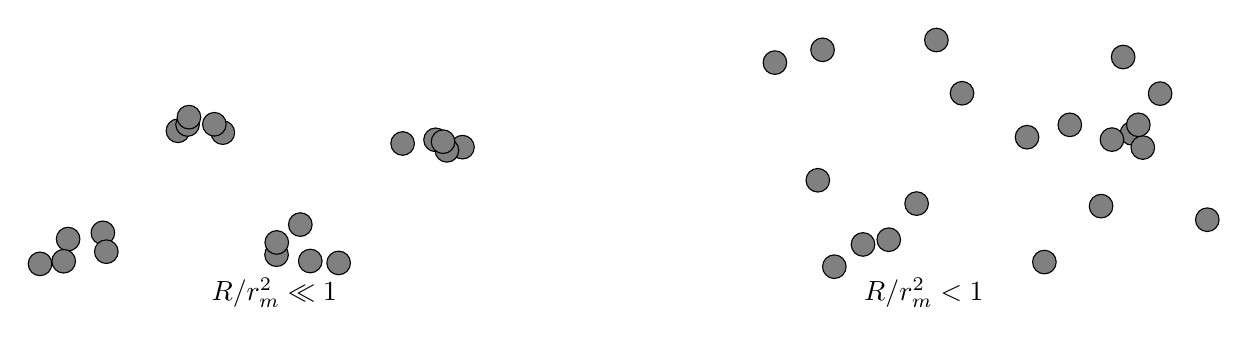
\begin{tikzpicture}[scale =1.5]
      
    \foreach \i in {1,...,5} {
    \pgfmathsetmacro{\x}{rnd*0.7}
    \pgfmathsetmacro{\y}{rnd*0.3}
    \draw[fill=gray] ($(\x,\y)$) circle (0.1);
    }
    \foreach \i in {1,...,5} {
    \pgfmathsetmacro{\x}{rnd*0.7}
    \pgfmathsetmacro{\y}{rnd*0.3}
    \draw[fill=gray] ($(\x+2,\y)$) circle (0.1);
    }
    \foreach \i in {1,...,5} {
    \pgfmathsetmacro{\x}{rnd*0.6}
    \pgfmathsetmacro{\y}{rnd*0.4}
    \draw[fill=gray] ($(\x+1,\y-1)$) circle (0.1);
    }
    \foreach \i in {1,...,5} {
    \pgfmathsetmacro{\x}{rnd*0.6}
    \pgfmathsetmacro{\y}{rnd*0.4}
    \draw[fill=gray] ($(\x-1,\y-1)$) circle (0.1);
    }
    \draw (1,-1)node[below]{$\mathbb{R}/r_m^2 \ll 1$};
  
      \foreach \i in {1,...,20} {
        \pgfmathsetmacro{\x}{rnd*4}
        \pgfmathsetmacro{\y}{rnd*2}
        \draw[fill=gray] ($(\x+5,\y-1)$) circle (0.1);
        }
        \draw (6.5,-1)node[below]{$\mathbb{R}/r_m^2 < 1$};
      \end{tikzpicture}
      \hfill
  \end{figure}
Let $\mathcal{R}_p^* = r_m^2 \textbf{I}$ being the isotropic microscale representation at random. 
It can be computed from the random distribution funciton $P_{nst}(\textbf{r}) =     P_{nst}(\textbf{x},\textbf{r})
= n_p e^{-4\pi n_p [r^3- (d)^3]/3}$ \citep{zhang2021ensemble}. 
Therefore, we have, 
\begin{equation}
    r_m^2 \textbf{I}
    = \int_{|\textbf{r}| > d}
    n_p(\textbf{x},t) \textbf{rr} e^{-4\pi n_p(\textbf{x},t) [|\textbf{r}|^3- (d)^3]/3}
    d\textbf{r}
\end{equation}
Since this quantity is isotropic let's focus on the $zz$ components using the change of variable : 
\begin{equation*}
    \textbf{r} = 
    \left\{
        \begin{tabular}{cc}
            $x =$&$ r \sin\theta \cos\phi$\\
            $y =$&$ r \sin\theta \sin\phi$\\
            $z =$&$ r \cos\theta$
        \end{tabular}
    \right.
\end{equation*}
Thus, the previous integral reads, 
\begin{align*}
    r_m^2 
    &= n_p \int_{0}^{2\pi}\int_{0}^{\pi}\int_{d}^{\infty}
     r^4 \cos^2\theta\sin\theta e^{-4\pi n_p [r^3- (d)^3]/3}
    drd\theta d\phi\\
    &= n_p \int_{0}^{2\pi}d\phi 
    \int_{0}^{\pi} \cos^2\theta\sin\theta d\theta 
    \int_{d}^{\infty}
     r^4  e^{-4\pi n_p [r^3- (d)^3]/3} dr\\
    &= n_p \pi
    \frac{4}{3} 
    e^{-4\pi n_p d^3 /3}
    \int_{d}^{\infty}
     r^4  e^{-4\pi n_p r^3 /3}
      dr\\
\end{align*}
Since this last integral isn't computable we will use $u = r^3$ thus $du = 3 r^2 dr$ or $dr = \frac{u^{-2/3}}{3} du$
\begin{equation*}
    \int_{d}^{\infty}
     r^4  e^{-4\pi n_p r^3 /3}
      dr
      = \frac{1}{3} 
      \int_{d^{1/3}}^{\infty}
        u^{2/3}  e^{-4\pi n_p u /3}
      du
      = \frac{1}{3}\left.
        -\frac{\Gamma(\frac{5}{2}, 4\pi n_p/3 u )}{(4\pi n_p/3)^{5/3}}
        \right|_{d^{1/3}}^\infty
      = 
        \frac{\Gamma(\frac{5}{2}, 4\pi n_p/3 d^{1/3} )}{3(4\pi n_p/3)^{5/3}}
\end{equation*}
The final results reads as,
\begin{equation*}
    r_m^2 =
    \frac{4n_p \pi e^{-4\pi n_p d^3 /3}}{9(4\pi n_p / 3)^{5/3}}
    \Gamma\left(\frac{5}{2}, 4\pi n_p d^{1/3} / 3 \right)
\end{equation*}
However this results is true if and only if we are in a dilute regime since it is under this assumption that $P_{nst}$ is defined. 
In practice for $\lambda = 1$ we recover this behavior. 


\subsection{Kinematics between particles}
voinoid cells here
\subsection{Dynamic between particles}
particle stress here
\subsection{Energy}
Compute the inter particle energy and the link of $ww$ with $<u'u'>$ 

\section{Some comments on the interaction force}
\begin{align}
    \textbf{f}_p (\textbf{x},t) &= \
    \frac{1}{n_p}\int \sum_i \delta(\textbf{x} - \textbf{x}_\alpha(t,\CC)) \textbf{f}_\alpha d\PP\\
    \label{eq:f_alpha}
    \text{with} \;\;\; &\textbf{f}_\alpha(t,\CC) = \int_{S_\alpha} (\bm{\sigma}_c^0(\textbf{x},t,\CC) - \bm{\sigma}_c(\textbf{x},t) )\cdot \textbf{n} dS \\
\end{align}
How does $\textbf{f}_\alpha$ evolve according to the presence of a particle ? 
In stokes flow for solid particle for exemple, 
\begin{equation}
    \textbf{f}_\alpha
    = - 6 \pi a \mu [
        \textbf{u}_\alpha(\CC,t)
        - \textbf{u}_c(\textbf{x},\CC',t)
        + \frac{1}{6}a^2 \nablab^2\textbf{u}_c(\textbf{x},\CC',t)
        - \textbf{W}
    ]
\end{equation}
where $\CC'$ correspond to the flow configuration $\CC$ whiteout the particle $\alpha$. 
\section{Dispersed phase fluctuations}
\todo[inline]{Explain how the dispersed phase fluctuation are related to the particles relative motions ?????}
\begin{equation}
    \textbf{u}_k
    = \int \nstavg{\chi_k \textbf{u}_k^0} P_{nst}(\textbf{x},\textbf{r},a,t)d\textbf{r}
\end{equation}
So does, 
\begin{equation}
    \textbf{u}'(\textbf{x},\CC,t)
    =\nstavg{ \textbf{u}^0}(\textbf{x},\textbf{r},t,a)' 
    = \nstavg{ \textbf{u}^0}(\textbf{x},\textbf{r},t,a) - \textbf{u}_k
\end{equation}
There is strong evidence that it is not true but show that :
\begin{equation}
    \avg{\textbf{u}'\textbf{u}'}(\textbf{x},\CC,t)
    =\int{ (\nstavg{ \textbf{u}^0} )'(\nstavg{ \textbf{u}^0})' }d\textbf{r}
    = \nstavg{ \textbf{u}^0} - \textbf{u}_k
\end{equation}
\subsubsection*{Continuous}
\begin{equation*}
    \textbf{u}(\textbf{x},t)
    = \int \nstavg{ \textbf{u}^0}  P_{nst}(\textbf{x},t,\textbf{r}) d\textbf{r}
    = \int  \textbf{u}^0(\textbf{x},t,\CC) d\PP 
\end{equation*}
Thus, 
\begin{equation*}
    \avg{\textbf{u}'\textbf{u}'}(\textbf{x},t)
    = \int \nstavg{ \textbf{u}^0 \textbf{u}^0}  
    P_{nst}(\textbf{x},t,\textbf{r}) d\textbf{r}
    - \textbf{uu}
    = \int  \textbf{u}^0\textbf{u}^0(\textbf{x},t,\CC) d\PP 
    - \textbf{uu}
\end{equation*}
Besides, if we note $\textbf{v}^0  =  \textbf{u}^0  - \nstavg{\textbf{u}}$
\begin{equation*}
    \avg{\textbf{u}'\textbf{u}'}(\textbf{x},t)
    + \textbf{uu}
    = \int 
    \nstavg{\textbf{u}^0} \nstavg{\textbf{u}^0} 
    P_{nst}(\textbf{x},t,\textbf{r}) d\textbf{r}
    +\int 
    \nstavg{ \textbf{v}^0\textbf{v}^0}  
    P_{nst}(\textbf{x},t,\textbf{r}) d\textbf{r}
\end{equation*}

For a phase averaged quantity it reads, 
\begin{equation*}
    \phi_k \textbf{u}_k(\textbf{x},t)
    = \int \nstavg{\chi_k \textbf{u}_k^0}  P_{nst}(\textbf{x},t,\textbf{r}) d\textbf{r}
    = \int  \chi_k \textbf{u}^0_k(\textbf{x},t,\CC) d\PP 
\end{equation*}
Thus similarly we have, 
\begin{equation*}
    \avg{\chi_k \textbf{u}'_k\textbf{u}'_k}(\textbf{x},t)
    = \int \nstavg{\chi_k \textbf{u}_k^0\textbf{u}_k^0}  P_{nst}(\textbf{x},t,\textbf{r}) d\textbf{r}
    - \phi_k \textbf{u}_k\textbf{u}_k
    = \int  \chi_k \textbf{u}^0_k\textbf{u}^0_k(\textbf{x},t,\CC) d\PP 
    - \phi_k \textbf{u}_k\textbf{u}_k
\end{equation*}
Introducing, $\textbf{v}_k^0  = \textbf{u}_k^0 - \nstavg{\chi_k \textbf{u}^0_k} / \nstavg{\chi_k}$
\begin{align*}
    \nstavg{\chi_k \textbf{u}_k^0\textbf{u}_k^0} 
    &= 
    \nstavg{\chi_k (\nstavg{\chi_k \textbf{u}^0_k} / \nstavg{\chi_k} + \textbf{v}_k^0)(\nstavg{\chi_k \textbf{u}^0_k} / \nstavg{\chi_k} + \textbf{v}_k^0)} \\
    &= 
    \nstavg{\chi_k} (\nstavg{\chi_k \textbf{u}^0_k}  \nstavg{\chi_k \textbf{u}^0_k} / (\nstavg{\chi_k})^2 
    + \nstavg{\chi_k \textbf{u}^0_k} \nstavg{\chi_k\textbf{v}_k^0}/ \nstavg{\chi_k}
    + \nstavg{\chi_k\textbf{v}_k^0} \nstavg{\chi_k \textbf{u}^0_k} / \nstavg{\chi_k}
    + \nstavg{\chi_k \textbf{v}_k^0\textbf{v}_k^0}
    )\\
    &= 
     (\nstavg{\chi_k \textbf{u}^0_k}  \nstavg{\chi_k \textbf{u}^0_k} / (\nstavg{\chi_k})
    + \nstavg{\chi_k \textbf{v}_k^0\textbf{v}_k^0}
    )\\
\end{align*}
Consequently, 
\begin{equation*}
    \avg{\chi_k \textbf{u}'_k\textbf{u}'_k}(\textbf{x},t)
    + \phi_k \textbf{u}_k\textbf{u}_k
    = 
    \int (\nstavg{\chi_k \textbf{u}^0_k}  \nstavg{\chi_k \textbf{u}^0_k} / (\nstavg{\chi_k})  P_{nst}(\textbf{x},t,\textbf{r}) d\textbf{r}
    +\int \nstavg{\chi_k \textbf{v}_k^0\textbf{v}_k^0}  P_{nst}(\textbf{x},t,\textbf{r}) d\textbf{r}
\end{equation*}

\subsubsection*{Particular}
Now we assume a pairwise nearest averaging process. 
On thing for sure : 
\begin{equation*}
    n_p \textbf{u}_p(\textbf{x},t)
    = \int \nstavg{ \textbf{u}^\alpha}  P_{nst}(\textbf{x},t,\textbf{r}) d\textbf{r}
    = \int  \textbf{u}_\alpha \delta_\alpha (\textbf{x},t,\CC) d\PP 
\end{equation*}
But also, 
\begin{equation*}
    n_p \textbf{u}_p \textbf{u}_p
    + \pavg{\textbf{u}_\alpha' \textbf{u}_\alpha'}
    =
    \int \nstavg{ \textbf{u}^\alpha\textbf{u}^\alpha}  P_{nst}(\textbf{x},t,\textbf{r}) d\textbf{r}
    = \int  \textbf{u}^\alpha\textbf{u}^\alpha \delta^\alpha (\textbf{x},t,\CC) d\PP 
\end{equation*}
If we introduce $\textbf{v}^\alpha = \textbf{u}^\alpha - \nstavg{\textbf{u}^\alpha}(\textbf{x},\textbf{r})$ 
\begin{equation*}
    \nstavg{ \textbf{u}^\alpha\textbf{u}^\alpha}
    = \nstavg{ (\textbf{v}^\alpha + \nstavg{\textbf{u}^\alpha})(\textbf{v}^\alpha + \nstavg{\textbf{u}^\alpha})}
    = \nstavg{ \textbf{u}^\alpha}\nstavg{\textbf{u}^\alpha} + \nstavg{ \textbf{v}^\alpha \textbf{v}^\alpha }(\textbf{x},\textbf{r})
\end{equation*}
The conclusion is that 
\begin{align*}
    n_p \textbf{u}_p \textbf{u}_p
    + \pavg{\textbf{u}_\alpha' \textbf{u}_\alpha'}
    =\int \nstavg{ \textbf{u}^\alpha}\nstavg{\textbf{u}^\alpha} P_{nst} d\textbf{r}
    + \int \nstavg{ \textbf{v}^\alpha \textbf{v}^\alpha }  P_{nst} d\textbf{r}\\
\end{align*}
thus the global fluctuation is the mean fluctuation plus the fluctuation at the position $(\textbf{x},\textbf{r})$. 

If we make the  good hypothesis the second integral might be negligible. 
Anyhow 

\section{Conclusion}
\bibliography{Bib/bib_bulles.bib}



\appendix

\end{document}
